\documentclass[11pt,a4paper]{article}
\usepackage[margin=1in]{geometry}
\usepackage{amsmath,amssymb}
\usepackage{graphicx}
\usepackage{enumitem}
\usepackage{tcolorbox}
\usepackage{array}
\usepackage{multirow}
\usepackage{tikz}
\usepackage{xcolor}
\usepackage{hyperref}
\usetikzlibrary{positioning,arrows.meta,shapes,calc}

% Colors
\definecolor{codegreen}{rgb}{0,0.6,0}
\definecolor{codegray}{rgb}{0.5,0.5,0.5}
\definecolor{codepurple}{rgb}{0.58,0,0.82}
\definecolor{backcolour}{rgb}{0.95,0.95,0.92}

% Custom commands
\newcommand{\highlight}[1]{\textbf{\color{blue}#1}}
\newcommand{\answer}[1]{\underline{\hspace{#1}}}
\newcommand{\checkbox}{$\Box$}

% Environment definitions
\newtcolorbox{exercise}[1][]{
    colback=blue!5!white,
    colframe=blue!75!black,
    title=#1,
    fonttitle=\bfseries
}

\newtcolorbox{checkpoint}[1][]{
    colback=yellow!10!white,
    colframe=orange!75!black,
    title=Checkpoint,
    fonttitle=\bfseries
}

\newtcolorbox{discovery}[1][]{
    colback=green!5!white,
    colframe=green!75!black,
    title=Discovery Moment,
    fonttitle=\bfseries
}

\newtcolorbox{think}[1][]{
    colback=purple!5!white,
    colframe=purple!75!black,
    title=Think About It,
    fonttitle=\bfseries
}

\newtcolorbox{realworld}[1][]{
    colback=orange!5!white,
    colframe=orange!75!black,
    title=Real World Application,
    fonttitle=\bfseries
}

\newtcolorbox{warning}[1][]{
    colback=red!5!white,
    colframe=red!75!black,
    title=Common Pitfall,
    fonttitle=\bfseries
}

% Title and header
\title{\textbf{Word Embeddings in 3D: Post-Class Learning Verification}\\
\large Checking Your Understanding After the Interactive Lab\\
\vspace{0.5em}
\large \textit{From Words to Vectors: Can You Apply What You Learned?}}
\author{NLP Course 2025 - BSc Level Assessment}
\date{}

\begin{document}
\maketitle

\noindent\textbf{Time Required:} 45-60 minutes\\
\textbf{Purpose:} Verify and deepen your understanding of word embeddings after completing the interactive notebook\\
\textbf{Format:} No coding required - focus on concepts, visualization, and application

\begin{checkpoint}
\textbf{Before Starting:} You should have completed the ``word\_embeddings\_3d\_bsc.ipynb'' notebook. This handout will test your understanding of:
\begin{itemize}
    \item Why words need to be vectors
    \item How Word2Vec learns from context
    \item Word similarity and clustering
    \item Word arithmetic
    \item Applications of embeddings
\end{itemize}
\end{checkpoint}

\hrule
\vspace{1em}

\section*{Part A: Conceptual Understanding \hfill (20 minutes)}

\subsection*{A1: The Embedding Concept (5 minutes)}

\begin{exercise}[Why Vectors?]
\textbf{Question 1:} Explain in your own words why computers need word embeddings instead of just treating words as text strings.

\vspace{3cm}

\textbf{Question 2:} Draw simple 2D vectors for these words showing their relationships:
\begin{itemize}
    \item cat, dog, car
    \item Show which two should be closer together and why
\end{itemize}

\begin{center}
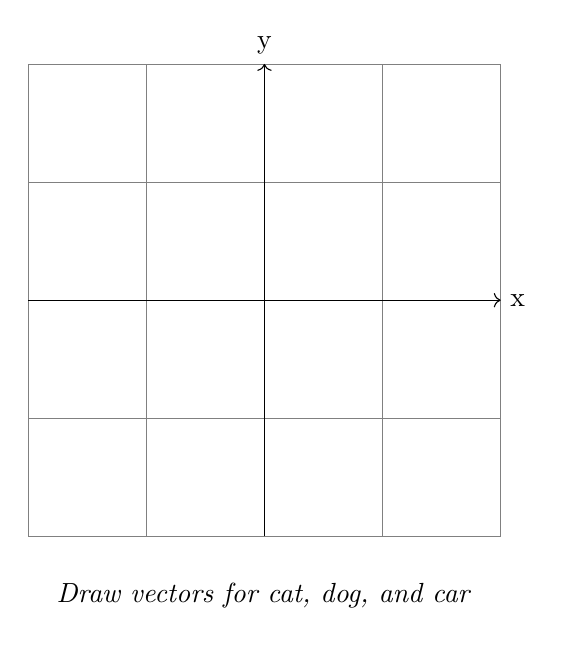
\begin{tikzpicture}[scale=1.5]
    % Grid
    \draw[gray, very thin] (-2,-2) grid (2,2);
    \draw[->] (-2,0) -- (2,0) node[right] {x};
    \draw[->] (0,-2) -- (0,2) node[above] {y};
    
    % Instructions
    \node at (0,-2.5) {\textit{Draw vectors for cat, dog, and car}};
\end{tikzpicture}
\end{center}

\textbf{Visualization:} Real 3D Word Embedding Space
\begin{center}
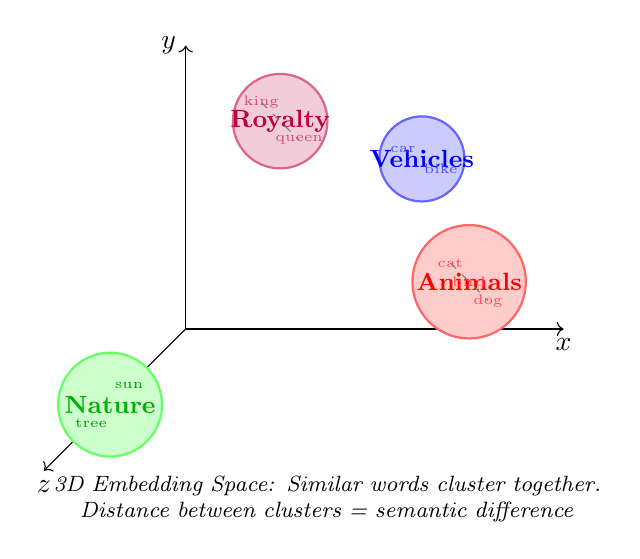
\begin{tikzpicture}[scale=1.2]
    % Pseudo-3D axes
    \draw[->] (0,0) -- (4,0) node[anchor=north]{$x$};
    \draw[->] (0,0) -- (0,3) node[anchor=east]{$y$};
    \draw[->] (0,0) -- (-1.5,-1.5) node[anchor=north]{$z$};
    
    % Animal cluster (red circle)
    \draw[red!60,fill=red!20,thick] (3,0.5) circle (0.6cm);
    \node[red,font=\small\bfseries] at (3,0.5) {Animals};
    \node[red!70,font=\tiny] at (2.8,0.7) {cat};
    \node[red!70,font=\tiny] at (3.2,0.3) {dog};
    \node[red!70,font=\tiny] at (3,0.5) {bird};
    
    % Royalty cluster (purple circle)  
    \draw[purple!60,fill=purple!20,thick] (1,2.2) circle (0.5cm);
    \node[purple,font=\small\bfseries] at (1,2.2) {Royalty};
    \node[purple!70,font=\tiny] at (0.8,2.4) {king};
    \node[purple!70,font=\tiny] at (1.2,2.0) {queen};
    
    % Nature cluster (green circle)
    \draw[green!60,fill=green!20,thick] (-0.8,-0.8) circle (0.55cm);
    \node[green!70!black,font=\small\bfseries] at (-0.8,-0.8) {Nature};
    \node[green!60!black,font=\tiny] at (-0.6,-0.6) {sun};
    \node[green!60!black,font=\tiny] at (-1.0,-1.0) {tree};
    
    % Vehicle cluster (blue circle)
    \draw[blue!60,fill=blue!20,thick] (2.5,1.8) circle (0.45cm);
    \node[blue,font=\small\bfseries] at (2.5,1.8) {Vehicles};
    \node[blue!70,font=\tiny] at (2.3,1.9) {car};
    \node[blue!70,font=\tiny] at (2.7,1.7) {bike};
    
    % Draw connections between similar words
    \draw[dashed,gray,thin] (2.8,0.7) -- (3.2,0.3);
    \draw[dashed,gray,thin] (0.8,2.4) -- (1.2,2.0);
    
    % Legend
    \node[font=\footnotesize,text width=7cm,align=center] at (1.5,-1.8) {
        \textit{3D Embedding Space: Similar words cluster together.\\
        Distance between clusters = semantic difference}
    };
\end{tikzpicture}
\end{center}

\textbf{Question 3:} Circle the TRUE statements:
\begin{itemize}
    \item[\checkbox] Embeddings capture word meaning as numbers
    \item[\checkbox] Similar words have similar vectors
    \item[\checkbox] Each word gets exactly one dimension
    \item[\checkbox] Context determines embedding values
    \item[\checkbox] Embeddings are always 3D
\end{itemize}
\end{exercise}

\subsection*{A2: Context Windows (5 minutes)}

\begin{exercise}[Understanding Context]
Given the sentence: \textbf{``The quick brown fox jumps over the lazy dog''}

\textbf{Task 1:} If we're training on the word ``fox'' with window size = 2, circle all context words:

\begin{center}
The \quad quick \quad brown \quad \boxed{fox} \quad jumps \quad over \quad the \quad lazy \quad dog
\end{center}

\textbf{Task 2:} How would changing window size affect learning?

\begin{tabular}{|l|p{8cm}|}
\hline
Window = 1 & \answer{8cm} \\
\hline
Window = 5 & \answer{8cm} \\
\hline
Window = 10 & \answer{8cm} \\
\hline
\end{tabular}

\textbf{Task 3:} Which window size would be better for:
\begin{itemize}
    \item Learning syntax (grammar): \answer{3cm}
    \item Learning topic/theme: \answer{3cm}
\end{itemize}
\end{exercise}

\subsection*{A3: Dimensions and Quality (5 minutes)}

\begin{exercise}[Dimension Trade-offs]
\textbf{Scenario:} You're choosing embedding dimensions for different applications.

\textbf{Task 1:} Match the dimension size to the use case:
\begin{center}
\begin{tabular}{|l|l|}
\hline
\textbf{Application} & \textbf{Suggested Dimensions} \\
\hline
Simple word similarity & \\
\hline
Complex language model & \\
\hline
Visualization in 3D & \\
\hline
Mobile app (limited memory) & \\
\hline
Research with huge vocabulary & \\
\hline
\end{tabular}
\end{center}

Options: 3, 10-50, 100-300, 500+, exactly 3

\textbf{Task 2:} Explain the trade-off:
\begin{itemize}
    \item More dimensions = \answer{5cm}
    \item Fewer dimensions = \answer{5cm}
\end{itemize}
\end{exercise}

\subsection*{A4: Quick Concept Check (5 minutes)}

\begin{think}
Rate your understanding (1 = confused, 5 = confident):
\begin{itemize}
    \item[\checkbox] Words as vectors \hfill [1] [2] [3] [4] [5]
    \item[\checkbox] Context windows \hfill [1] [2] [3] [4] [5]
    \item[\checkbox] Training process \hfill [1] [2] [3] [4] [5]
    \item[\checkbox] Similarity measurement \hfill [1] [2] [3] [4] [5]
\end{itemize}
\end{think}

\newpage

\section*{Part B: Practical Application \hfill (15 minutes)}

\subsection*{B1: Word Similarity Exercise (5 minutes)}

\begin{exercise}[Computing Similarity]
Given these simplified 3D embeddings:
\begin{itemize}
    \item king = [0.8, 0.2, 0.5]
    \item queen = [0.7, 0.3, 0.6]
    \item car = [0.1, 0.9, 0.2]
\end{itemize}

\textbf{Task 1:} Which pair is more similar? (Use rough estimation)
\begin{itemize}
    \item king \& queen: Distance $\approx$ \answer{2cm}
    \item king \& car: Distance $\approx$ \answer{2cm}
    \item More similar pair: \answer{3cm}
\end{itemize}

\textbf{Task 2:} Rank these word pairs by expected similarity (1 = most similar):
\begin{itemize}
    \item[\checkbox] cat - dog
    \item[\checkbox] king - queen
    \item[\checkbox] happy - sad
    \item[\checkbox] computer - laptop
    \item[\checkbox] run - blue
\end{itemize}

\textbf{Task 3:} Draw approximate clusters:
\begin{center}
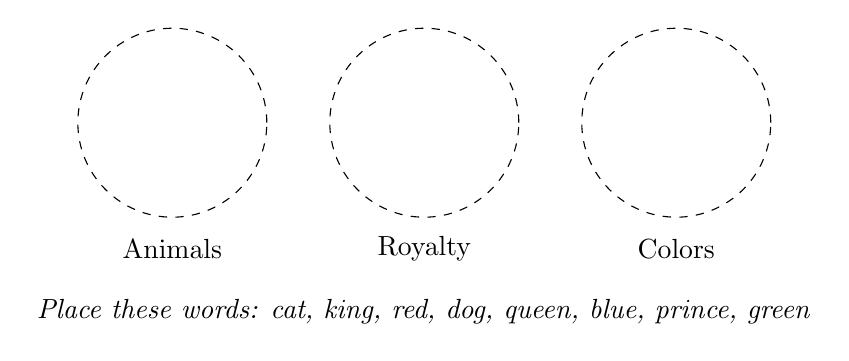
\begin{tikzpicture}[scale=0.8]
    % Draw circles for clusters
    \draw[dashed] (0,0) circle (1.5cm);
    \node at (0,-2) {Animals};
    
    \draw[dashed] (4,0) circle (1.5cm);
    \node at (4,-2) {Royalty};
    
    \draw[dashed] (8,0) circle (1.5cm);
    \node at (8,-2) {Colors};
    
    \node at (4,-3) {\textit{Place these words: cat, king, red, dog, queen, blue, prince, green}};
\end{tikzpicture}
\end{center}
\end{exercise}

\subsection*{B2: Word Arithmetic Magic (5 minutes)}

\begin{exercise}[Vector Math with Words]
\textbf{Task 1:} Complete these analogies:
\begin{itemize}
    \item king - man + woman = \answer{3cm}
    \item paris - france + germany = \answer{3cm}
    \item cat - kitten + puppy = \answer{3cm}
\end{itemize}

\textbf{Task 2:} Create your own word equation:

\answer{3cm} - \answer{3cm} + \answer{3cm} = \answer{3cm}

\textbf{Task 3:} Draw the vector arithmetic for: ``summer - hot + cold''

\begin{center}
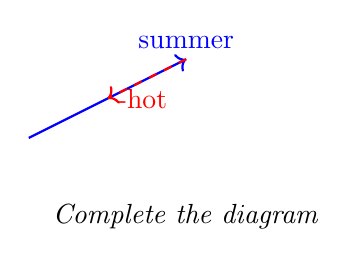
\begin{tikzpicture}[scale=1]
    % Start with summer vector
    \draw[->, thick, blue] (0,0) -- (2,1) node[above] {summer};
    
    % Subtract hot
    \draw[->, thick, red, dashed] (2,1) -- (1,0.5) node[right] {-hot};
    
    % Add cold (placeholder for student to complete)
    % \draw[->, thick, green] (1,0.5) -- (2.5,1.5) node[above] {+cold};
    
    % Result
    \node at (2,-1) {\textit{Complete the diagram}};
\end{tikzpicture}
\end{center}

\textbf{Task 4:} Explain why word arithmetic works:

\vspace{3cm}
\end{exercise}

\subsection*{B3: 3D Visualization Interpretation (5 minutes)}

\begin{exercise}[Reading 3D Plots]
Imagine you see a 3D plot where:
\begin{itemize}
    \item ``love'' and ``hate'' are far apart
    \item ``cat'' and ``dog'' are close together
    \item ``king'' and ``queen'' form a cluster with ``prince''
\end{itemize}

\textbf{Task 1:} What does distance represent in the plot?

\answer{8cm}

\textbf{Task 2:} Where would you expect to find these words?
\begin{itemize}
    \item ``affection'' - Near: \answer{3cm}
    \item ``princess'' - Near: \answer{3cm}
    \item ``fish'' - Near: \answer{3cm}
\end{itemize}

\textbf{Task 3:} If words gradually move closer during training, what's happening?

\answer{8cm}
\end{exercise}

\newpage

\section*{Part C: Hands-On Problem Solving \hfill (15 minutes)}

\subsection*{C1: Build Your Own Embeddings (5 minutes)}

\begin{exercise}[Design Embeddings from Scratch]
Given these 5 sentences:
\begin{enumerate}
    \item The cat sleeps
    \item The dog plays
    \item Cats and dogs play
    \item Birds fly high
    \item Fish swim deep
\end{enumerate}

\textbf{Task 1:} Create word-context pairs for ``cat'' (window=1):
\begin{itemize}
    \item Context words: \answer{5cm}
    \item Context words: \answer{5cm}
\end{itemize}

\textbf{Task 2:} Design simple 2D vectors for these words:
\begin{center}
\begin{tabular}{|l|c|c|}
\hline
\textbf{Word} & \textbf{x} & \textbf{y} \\
\hline
cat & & \\
\hline
dog & & \\
\hline
bird & & \\
\hline
fish & & \\
\hline
\end{tabular}
\end{center}

\textbf{Task 3:} Which words should cluster together? Why?

\answer{8cm}
\end{exercise}

\subsection*{C2: Application Design (5 minutes)}

\begin{exercise}[Building with Embeddings]
\textbf{Task 1:} Design a synonym finder:

\begin{enumerate}
    \item Input: \answer{4cm}
    \item Process: \answer{6cm}
    \item Output: \answer{4cm}
\end{enumerate}

\textbf{Task 2:} Sketch a sentiment analyzer:

How would you use embeddings to determine if text is positive/negative?

\vspace{3cm}

\textbf{Task 3:} Your creative application:

Design a new use for word embeddings:
\begin{itemize}
    \item Name: \answer{5cm}
    \item Purpose: \answer{8cm}
    \item How embeddings help: \answer{8cm}
\end{itemize}
\end{exercise}

\subsection*{C3: Debugging Scenarios (5 minutes)}

\begin{warning}
Real problems you might encounter:
\end{warning}

\begin{exercise}[Problem Solving]
\textbf{Scenario 1:} The word ``bank'' appears near both ``river'' and ``money''. 
\begin{itemize}
    \item Problem: \answer{6cm}
    \item Solution: \answer{6cm}
\end{itemize}

\textbf{Scenario 2:} A new word ``COVID'' doesn't exist in your embeddings.
\begin{itemize}
    \item Problem: \answer{6cm}
    \item Solution: \answer{6cm}
\end{itemize}

\textbf{Scenario 3:} Your embeddings show ``doctor''=male, ``nurse''=female bias.
\begin{itemize}
    \item Problem: \answer{6cm}
    \item Solution: \answer{6cm}
\end{itemize}
\end{exercise}

\newpage

\section*{Part D: Reflection \& Extension \hfill (10 minutes)}

\subsection*{D1: Self-Assessment Checklist (3 minutes)}

\begin{checkpoint}
Check off what you can now do:
\begin{itemize}
    \item[\checkbox] Explain why words need to be vectors
    \item[\checkbox] Describe how Word2Vec learns from context
    \item[\checkbox] Calculate word similarity (roughly)
    \item[\checkbox] Perform word arithmetic
    \item[\checkbox] Identify word clusters in 3D space
    \item[\checkbox] Design applications using embeddings
    \item[\checkbox] Recognize common problems and solutions
\end{itemize}
\end{checkpoint}

\subsection*{D2: Real-World Connections (3 minutes)}

\begin{realworld}
\textbf{Connect to Industry:}
\begin{enumerate}
    \item How does Google use embeddings in search?
    
    \answer{8cm}
    
    \item How do embeddings connect to ChatGPT/BERT?
    
    \answer{8cm}
    
    \item Name one ethical concern with embeddings:
    
    \answer{8cm}
\end{enumerate}
\end{realworld}

\subsection*{D3: Challenge Questions (4 minutes)}

\begin{think}
\textbf{Going Deeper:}
\begin{enumerate}
    \item Could we create embeddings for images? How?
    
    \vspace{2cm}
    
    \item What about embedding DNA sequences or music?
    
    \vspace{2cm}
    
    \item How would you embed an entire document (not just words)?
    
    \vspace{2cm}
\end{enumerate}
\end{think}

\hrule
\vspace{1em}

\section*{Final Reflection}

\begin{discovery}
\textbf{The Big Picture:}

You've learned that word embeddings transform language into mathematical space where:
\begin{itemize}
    \item Meaning becomes measurable
    \item Relationships become computable
    \item Patterns become visible
\end{itemize}

This is the foundation of modern NLP - from search engines to chatbots to translation systems!
\end{discovery}

\vspace{1em}

\textbf{Areas needing review?} List them here:
\begin{itemize}
    \item \answer{8cm}
    \item \answer{8cm}
    \item \answer{8cm}
\end{itemize}

\vspace{1em}

\textbf{Most interesting discovery:} \answer{10cm}

\vspace{1em}

\textbf{One question you still have:} \answer{10cm}

\hrule
\vspace{1em}

\section*{Next Steps}

\begin{itemize}
    \item Review sections with ratings below 3
    \item Try coding your own Word2Vec model
    \item Explore pre-trained embeddings (GloVe, FastText)
    \item Learn about contextual embeddings (BERT)
    \item Apply embeddings to a real project
\end{itemize}

\vspace{2em}
\begin{center}
\textbf{--- End of Assessment ---}
\end{center}

\end{document}